\documentclass[11pt,a4paper]{article}
\usepackage[utf8]{inputenc}
\usepackage{a4wide}
\usepackage{fancyhdr}
\usepackage{pdfpages}
\usepackage{listings}
\pagestyle{fancy}
\thispagestyle{fancy}

\usepackage{gensymb}
\usepackage{hyperref}
\newcommand\fnurl[2]{%
  \href{#2}{#1}\footnote{\url{#2}}%
}
\usepackage{amsfonts}
% Bibliografía
\usepackage{natbib}

\usepackage[spanish]{babel}
\parskip = 11pt
\addtolength{\topmargin}{-1cm}
\addtolength{\textheight}{2.2cm}
\addtolength{\textwidth}{-.5cm}

\makeatletter
\renewcommand\paragraph{\@startsection{paragraph}{4}{\z@}%
            {-2.5ex\@plus -1ex \@minus -.25ex}%
            {1.25ex \@plus .25ex}%
            {\normalfont\normalsize\bfseries}}
\makeatother
\setcounter{secnumdepth}{4} % how many sectioning levels to assign numbers to
\setcounter{tocdepth}{4}    % how many sectioning levels to show in ToC

\usepackage[conEntregas]{caratula}
\materia{Teoría de las Comunicaciones}
\titulo{Trabajo Práctico II}
\subtitulo{\textit{Rutas en Internet}}
\integrante{Fernández, Gonzalo}{836/10}{gpfernandezflorio@gmail.com}
\integrante{Aleman, Damián Eliel}{377/10}{damianealeman@gmail.com}
\integrante{Pizzagalli, Matías}{257/12}{matipizza@gmail.com}

\begin{document}

\maketitle

\tableofcontents

\newpage

\section{Introducción Teórica}

\subsection{Modelo OSI}

El modelo OSI es un modelo que abstrae en 7 capas los protocolos involucrados en la comunicación entre dos nodos en una red.

\begin{center}
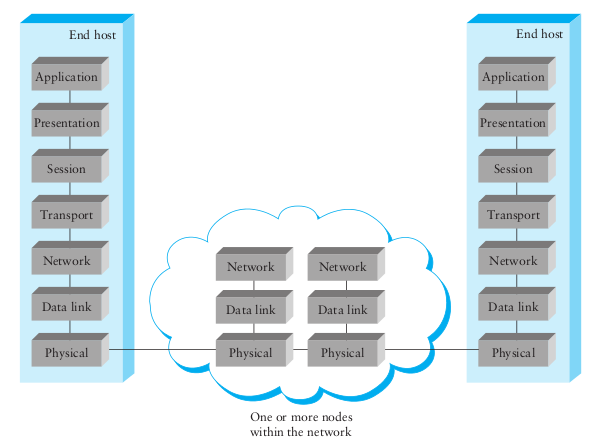
\includegraphics[width=\textwidth/2]{imgs/osi.png}
\end{center}

\subsection{Paquetes IP}

Los paquetes IP\footnote{RFC 791 (IP): https://tools.ietf.org/html/rfc791} son el método principal de intercambio de mensajes entre nodos a nivel de red. Es decir, cuando los nodos pertenecen a distintas redes locales y no tienen acceso la dirección física del otro. El protocolo IP es \textit{best-effort}, por lo tanto existe la posibilidad de que un mensaje nunca llegue a destino. Es más, los routers que implementan RED\footnote{RFC 2309 (RED): https://tools.ietf.org/html/rfc2309}, están configurados para descartar paquetes periódicamente con alguna probabilidad, incluso antes de entrar en un estado de congestión.

\subsection{Paquetes ICMP}

Los paquetes ICMP\footnote{RFC 792 (ICMP): https://tools.ietf.org/html/rfc792} son paquetes de control que no contienen datos, utilizados por los routers para reportar errores en el intercambio de mensajes de una conexión.

\subsection{Traceroute}

Traceroute es una herramienta que permite mostrar la ruta de una conexión entre dos nodos, identificando todos los nodos intermedios y sus respectivos tiempos de demora.


\section{Desarrollo}

Como estamos trabajando con paquetes IP, no tenemos asegurado que el paquete enviado llegue a destino, así como que la respuesta llegue de regreso. Debemos tener esto en cuenta al momento de hacer las mediciones.

Al suponer que la carga de la red de una región depende del horario, proponemos como hipótesis que los tiempos totales medidos diferirán según el horario en que se envían debido a distintos niveles de carga en las redes utilizadas. También es posible que esta diferencia no se vea en conexiones lejanas ya que podrían balancearse las demoras entre las distintas regiones. Esto se debe a que tienen distintos usos horarios, luego la carga se distribuye en el tiempo de otra forma.

La técnica de estimación de outliers sirve para identificar valores distantes en módulo a la media. Al utilizar esta técnica vamos a estar identificando valores muy por encima y muy por debajo de la media. Sin embargo, como el objetivo es identificar saltos intercontinentales, tendremos en cuenta sólo aquellos outliers por encima de la media, ya que estos presentan una gran distancia entre dos saltos consecutivos.


\section{Resultados}

Para experimentar con las herramientas desarolladas, realizamos traceroutes a IPs pertenecientes a sitios web de universidades en diferentes paises alrededor del mundo. De todas las epxerimentaciones que hicimos nos quedamos con tres universidades:
\begin{itemize}
  \item Lomonosov Moscu State University, situada en Moscu, Rusia, Europa. (\url{www.msu.ru})
  \item The University of Tokyo, situada en Tokio, Japon, Asia. (\url{www.u-tokyo.ac.jp})
  \item The University of Sydney, situada en Sydney, Australia, Oceania. (\url{www.sydney.edu.au})
\end{itemize}

\subsection{Lomonosov Moscu State University}
A continuación podemos observar los resultados que obtuvimos al probar nuestra herramiento de traceroute
con destino la universidad situada en Moscu, es decir \url{www.msu.ru}.

\begin{figure}[H]
\begin{center}
\begin{tabular}{|c|c|c|c|c|}
  \hline
  HOP & RTT & RTT RELATIVO & Ubicación & ZRTT \\ \hline
 192.168.1.1 & 66 ms & 0 & - & -0,2714373843 \\ \hline
 10.21.192.1 & 75 ms & 9 & - & -0,160394818 \\ \hline
 10.242.1.17 & 80 ms & 5 & - & -0,2097470697 \\ \hline
 208.178.195.210 & 84 ms & 4 & (Estados Unidos) & -0,2220851326 \\ \hline
 208.178.195.209 & 91 ms & 7 & (Estados Unidos) & -0,1850709439 \\ \hline
 * & & & & \\ \hline
 4.69.158.253 & 335 ms & \textbf{244} & Suecia & \textbf{2,739049969} \\ \hline
 4.69.158.253 & 329 ms & -6 & Suecia & -0,3454657619 \\ \hline
 213.242.110.198 & 356 ms & 27 & (Reino Unido) & 0,06169031462 \\ \hline
 * & & & & \\ \hline
 194.85.40.229 & 462 ms & 106 & (Rusia) & 1,036397286 \\ \hline
 194.190.254.118 & 378 ms & -84 & (Rusia) & -1,30783467 \\ \hline
 93.180.0.172 & 464 ms & 86 & Moscu (Rusia) & 0,7896360271 \\ \hline
 188.44.33.30 & 439 ms & -25 & Moscu (Rusia) & -0,5798889574 \\ \hline
 188.44.33.2 & 365 ms & -74 & Moscu (Rusia) & -1,184454041 \\ \hline
 188.44.50.103 & 383 ms & 18 & Moscu (Rusia) & -0,0493522517 \\ \hline
% \hline
%  & Average: & 22 & & & \\
%  & Std Deviation: & 81.0555365166 & & & \\
%  & Outlier: & 4.69.158.253 & & & \\
% \hline

\end{tabular}


Además obtuvimos mediante la técnica de estimación de outliers el salto desde Estados Unidos (208.178.195.209) hacia Suecia (4.69.158.253). Efectivamente ese es un salto transcontinental. 
En el siguiente gráfico podemos observar las variaciones de ZRTT a lo largo de los saltos de la ruta:


\caption{Tabla generada por Traceroute a la Universidad de Moscu (188.44.50.103)}
% \label{my-label}
\end{center}
\end{figure}

Podemos observar en el gráfico que además del salto identificado mediante la técnica de Cimbala, sobresalen también el salto desde el Reino Unido hasta Rusia. Aquí se observa la ventaja de este método gráfico y la efectividad del método de Cimbala. 

\begin{center}
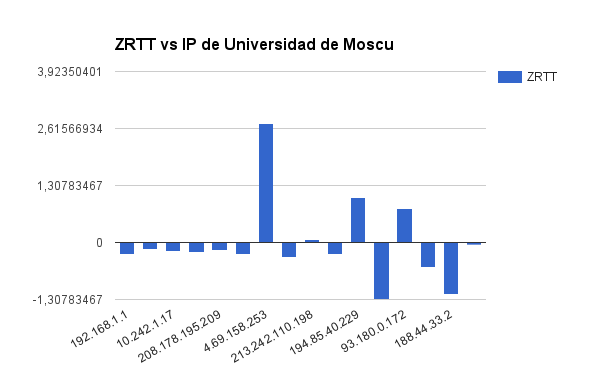
\includegraphics[width=\textwidth]{imgs/moscu.png}
\end{center}


\subsection{The University of Tokyo}
Acontinuación mostramos los resultados obtenidos cuando tomamos como destino la
Universidad de Tokio, es decir \url{www.u-tokyo.ac.jp}.

\begin{figure}[H]
\begin{center}
\begin{tabular}{|c|c|c|c|c|}
  \hline
  HOP & RTT & RTT RELATIVO & Ubicación & ZRTT \\ \hline
  192.168.1.1 & 62 ms & 0 & - & -0,3018867925 \\ \hline
  10.21.192.1 & 159 ms &  97  & - &  1,528301887 \\ \hline
  10.242.1.17 & 123 ms &  -36 & - & -0,9811320755 \\ \hline
  195.22.220.33 & 76 ms & -47 & (Italia) & -1,188679245 \\ \hline
  195.22.220.32 & 127 ms &  51  & (Italia)&  0,6603773585 \\ \hline
  195.22.219.145 &  160 ms &  33  & (Italia)&  0,320754717 \\ \hline
  195.22.219.145 &  95 ms & -65 & (Italia) & -1,528301887 \\ \hline
  149.3.181.65 &  106 ms &  11  & (Italia) & -0,09433962264 \\ \hline
  129.250.2.227 & 222 ms &  116 & Englewood (Estados Unidos)&  1,886792453 \\ \hline
  129.250.4.13 &  272 ms &  50  & Englewood (Estados Unidos)&  0,641509434 \\ \hline
  129.250.2.54 &  269 ms &  -3  & Englewood (Estados Unidos) & -0,358490566 \\ \hline
  129.250.3.86 &  418 ms &  \textbf{149} & Englewood (Estados Unidos)&  \textbf{2,509433962} \\ \hline
  129.250.6.188 & 405 ms &  -13 & Englewood (Estados Unidos) & -0,5471698113 \\ \hline
  129.250.2.255 & 404 ms &  -1  & Englewood (Estados Unidos) & -0,320754717 \\ \hline
  61.200.80.218 & 396 ms &  -8  & (Japón) & -0,4528301887 \\ \hline
  158.205.192.173 & 414 ms &  18  & (Japón)&  0,03773584906 \\ \hline
  158.205.192.86 &  413 ms &  -1  & (Japón) & -0,320754717 \\ \hline
  158.205.121.250 & 387 ms &  -26 & (Japón) & -0,7924528302 \\ \hline
  154.34.240.254 &  407 ms &  20  & (Japón)&  0,07547169811 \\ \hline
  210.152.135.178 & 399 ms &  -8  & (Japón) & -0,4528301887 \\ \hline
\end{tabular}
\caption{Tabla generada por Traceroute a la Universidad de Tokyo (210.152.135.178)}
% \label{my-label}
\end{center}
\end{figure}


\begin{center}
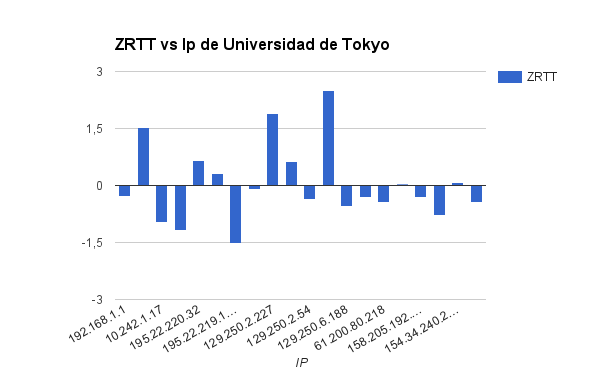
\includegraphics[width=\textwidth]{imgs/tokyo.png}
\end{center}


\subsection{The University of Sydney}
A continuacion podemos observar los resultados que obtuvimos al probar nuestra herramiento de traceroute
con destino \url{www.sydney.edu.au}.

\begin{figure}[H]
\begin{center}
\begin{tabular}{|c|c|c|c|c|}
  \hline
  HOP & RTT & RTT RELATIVO & Ubicación & ZRTT \\ \hline
  192.168.1.1     & 83 ms  & 0          & - & -0,3940627873 \\ \hline
  10.21.192.1     & 167 ms & 84         & - & 0,7093130172  \\ \hline
  10.242.1.17     & 83 ms  & -84        & - & -1,497438592  \\ \hline
  195.22.220.33   & 67 ms  & -16        & - & -0,6042296073 \\ \hline
  195.22.220.32   & 78 ms  & 11         & - & -0,2495730986 \\ \hline
  195.22.206.190  & 270 ms & \textbf{192}        & - & \textbf{2,127939052}   \\ \hline
  198.32.176.177  & 312 ms & 42         & - & 0,1576251149  \\ \hline
  202.158.194.176 & 419 ms & 107        & - & 1,011427821   \\ \hline
  113.197.15.146  & 458 ms & 39         & - & 0,1182188362  \\ \hline
  138.44.5.47     & 416 ms & -42        & - & -0,9457506896 \\ \hline
  * * *           &        &            & - & -0,3940627873 \\ \hline
  * * *           &        &            & - & -0,3940627873 \\ \hline
  129.78.5.8      & 413 ms & -3         & - & -0,4334690661 \\ \hline
\end{tabular}
\caption{Tabla generada por Traceroute a la Universidad de Sydney (129.78.5.8)}
% \label{my-label}
\end{center}
\end{figure}


\begin{center}
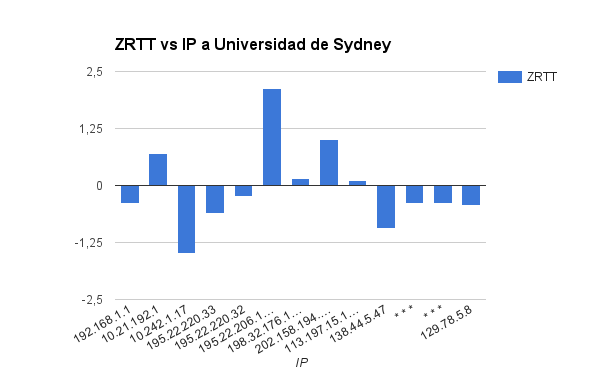
\includegraphics[width=\textwidth]{imgs/sydney.png}
\end{center}






\section{Conclusiones}

\section{Conclusiones.}

Si bien la tool diseñada y el método propuesto nos permiten obtener la ruta a un website detectando los posibles enlaces intercontinentales, este procedimiento está sujeto a numerosas adversidades. Routers que no responden (aún con timeouts largos) o que asignan prioridad baja a los paquetes ICMP,  geolocalizadores inexactos, congestión en una ruta o rutas distintas para un mismo website son mayormente lo que notamos que afecta considerablemente a los resultados obtenidos.  Veamos algunas de estas problemáticas en detalle:

En los casos en los que no obtenemos una respuesta del router, no tenemos forma de conocer, con este método, esa parte de la ruta, aún sabiendo que allí debería haber un nodo. Esto afecta a la comparativa general ya que, en caso de tener numerosas no-respuestas sucesivas, el RTT relativo entre los extremos de esta secuencia podría distribuirse de diversos modos. Un caso posible consiste en una distribución equitativa de los RTTs entre los nodos de la secuencia significando que ninguno corresponde a un enlace submarino. A su vez podría suceder que la distribución sea desigual y exista un enlace intermedio de elevado RTT representando una conexión intercontinental.

Por otra parte, en los casos en donde obtenemos una respuesta, esta información no necesariamente basta. La estimación de la distancia entre hops mediante el RTT no resulta demasiado confiable debido a que el tiempo de ida y vuelta (de la forma calculada) no depende única y exclusivamente de la longitud del enlace sino también incluye el tiempo del paquete dentro del router que podría extenderse por congestión, prioridad u otros factores. Además la congestión a lo largo de la red puede no ser uniforme a lo largo de la ruta en un momento dado y cada router puede tener una asignación de prioridades diferente. De esta manera la comparación entre RTTs se ve afectada no sólo por el momento de la medición sino tambien por los nodos involucrados en la ruta elegida. Una forma posible de resolver la congestión en un horario podría ser tomar mediciones en distintos momentos del día, pudiendo así tener una idea de cómo afecta la congestión a nuestras mediciones.

A pesar de esto, encontramos casos en los que el método pudo ser llevado a cabo de forma efectiva.


\newpage

\section{Apéndice}

\input{apendice.tex}

\end{document}
